\documentclass[prb,11pt]{revtex4-1}

% preamble:

\usepackage{amsmath}    % need for subequations
\usepackage{graphicx}   % need for figures
\usepackage{verbatim}   % useful for program listings
\usepackage{color}      % use if color is used in text
\usepackage{subfigure}  % use for side-by-side figures
\usepackage{hyperref}   % use for hypertext links, including those to external documents and URLs
\raggedbottom           % don't add extra vertical space
\begin{comment}
\pagestyle{empty}       % use if page numbers not wanted
\end{comment}

\begin{document}

\title{Effective viscosity of polymer networks in the presence of cross-link slip}
\author{William McFadden}
\affiliation{University of Chicago, Biophysical Sciences Program, Chicago, IL 60615}

\date{1 January 2014}

\begin{abstract}
We are trying to describe the problem of what happens when cross-links relax stress in semi-flexible filament networks.  We have addressed the problem using a simplified model in which cross-links are allowed to slip past one another in a friction-like manner.  This model gives a prediction for the long timescale effective viscosity of the medium.  We have verified our solution using computational models of filaments in the limit where persistence length is much longer than filament length.  In this model, we find that network architectures and slip rates give rise to different modes of connectivity.
\end{abstract}

\maketitle

\section{Introduction}

In previous work, crosslinks have been taken to be either perfectly rigid attachment points (HLM) or extended springlike structures (Taeyoon).  In addition, any mechanism of detachment is either absent (HLM) or governed by full detachment and full reattachment events (Taeyoon, Broederz).  In our model, we aim to create a more simple picture of crosslink stress relaxation based on an effective molecular friction between filament attachment points.

Previous researchers have introduced the concept of molecular friction to describe crosslink slip.  We want to look at what such a model would produce in a larger network.

Chemists have made synthetic systems that exhibit so called slide-ring cross-linking, but thus far this exact mechanism has not been seen in biological systems.  However, (some garbage experiments from biophysical journal that I know must exist because people put bullshit in biophysical journal all the time) have shown that multivalent crosslinks can effectively slide under a load.


\section{The Model}

In the worm-like chain model, semi-flexible polymers are modeled as continuous curves, governed by a potential 
\begin{equation}
{\cal H} =\frac{1}{2}\kappa \int ds(\nabla^2\mathbf{u})^2 + \frac{1}{2}\mu \int ds \left ( \frac{dl(s) }{ds} \right )^2
\end{equation}

We generate 2D networks of these semi flexible filaments by laying them down with random position and orientation.  

Although real cytoskeletal networks may exhibit non-negligible anisotropy, we choose to focus our attention on isotropic networks for simplicity.  We define the density using the . A simple geometrical argument can be used to prove that the number of filaments needed to fill a domain of size 2D x D is $4D^2/Ll_c$. 

In the absence of crosslink slip, we expect the network to comprise a connected solid with a well defined elastic modulus given by HLM.  

In departure from the previous models we wish to incorporate relaxation of the networks stored stress by letting the attachment points slip.  We do this by introducing a frictional coupling between filaments.
\begin{equation}
\mathbf{F_{friction}} = \delta \zeta \cdot \int ds \: (\mathbf{v(s)}-\mathbf{v_0(s)}) \: p(s)
\end{equation}

In this case the motion for the entire network is governed by a dynamical equation of the form

\begin{equation}
\zeta \int ds \: (\mathbf{v_i(s)} + \delta \sum _j(\mathbf{v_i(s)}-\mathbf{v_j(s)}) \: p_{ij}(s))= \nabla {\cal H}_i
\end{equation}

Although the general mechanical response of this system may be very complex, we wish to focus our attention on the linear order steady-state creep response of the system to an applied stress.  To do this we introduce a spatially varying stress along the midline of our domain.

\begin{equation}
F_{total}= \nabla {\cal H}_i + \sigma(x)-\zeta \int ds \: (\mathbf{v_i(s)} + \delta \sum _j(\mathbf{v_i(s)}-\mathbf{v_j(s)}) \: p_{ij}(s)) 
\end{equation}

Finally, we add a 0 velocity constraint at the far edges of our domain of interest.  We assume that our network is in the low Reynold's number limit, where inertial effects are so small that we can equate our total force to 0.  The above equation is then discretized and integrated in time to determine the material response.

\section{Analytical Results}
We would like to calculate an estimate of the effective viscosity for a network described by our model.  We carry this out by assuming we can apply a constant stress along a transect of the network.  With small stresses, we assume the network reaches a steady state affine creep. In this situation, we would find that the stress in the network exactly balances the sum of the frictional forces from crosslink slip.  So for any transect of length D, we have

\begin{equation}
\mathbf{\sigma} = \frac{1}{D}\sum_{filaments}\: \sum_{crosslinks}\delta \zeta \cdot (\mathbf{v_i}-\mathbf{v_0})\end{equation}

We can convert the sum over crosslinks to an integral over the length using the average density of crosslinks, $1/l_c$ and invoking the assumption of (linear order) affine strain rate, $\mathbf{v_i}-\mathbf{v_0}=\dot \gamma x$. This results in

\begin{equation}
\mathbf{\sigma} =  \frac{1}{D}\sum_{filaments}\:  \delta \zeta \cdot \int_0^L ds \: (\mathbf{v(s)}-\mathbf{v_0(s)}) \:\frac{1}{l_c} = \sum_{filaments}\:  \frac{\delta \zeta \dot \gamma L}{l_c} \cos \theta \cdot (x_l + \frac{L}{2} \cos \theta)
\end{equation}

Here we have introduced the variables $x_l$, and $\theta$ to describe the leftmost endpoint and the angular orientation of a given filament.  Next, to perform the sum over all filaments we wish to convert this to an integral over all orientations and endpoints that intersect our line of stress. The max distance for the leftmost endpoint is L, and the maximum angle as a function of endpoint is $\arccos(x_l/L)$.  The linear density of endpoints is the constant $D/l_cL$ so our integrals can be rewritten as this density over $x_l$ and $\theta$ between our maximum and minimum allowed bounds.

\begin{equation}
\mathbf{\sigma} =  \frac{1}{D} \int_0^L dx_l \int_{-\arccos (\frac{x_l}{L})}^{\arccos (\frac{x_l}{L})}d\theta \frac{\delta \zeta \dot \gamma L}{l_c} \cdot \frac{D}{Ll_c}\cdot (x_l \cos \theta + \frac{L}{2} cos^2\theta)
\end{equation}

Carrying our the integrals leaves us with a relation between stress and strain rate

\begin{equation}
\mathbf{\sigma} = \frac{4L^2\delta \zeta}{3l_c^2} \dot \gamma \end{equation}

which is reveals that the term next to the strain rate is the effective viscosity $\eta_{eff}$ at steady state creep.  With the constitutive relation for the rate of deformation, we can next write down an equation for the rate of network thinning.  

\begin{equation}
\frac{\partial l_c}{dt}=l_c\dot \gamma =\frac{l_c \sigma}{\eta}=l_c^3\frac{ \sigma}{L^2 \delta \zeta}
\end{equation}

We can see that the rate of network thinning accelerates as we would expect.  When the network reaches some minimum connectivity we assume that it stops behaving as a continuum material.  

\begin{equation}
\tau_{break} = \frac{\eta_{eff}}{2\sigma}\cdot\left ( 1 -\frac{l_c^2}{l_{break}^2} \right )
\end{equation}

This provides us with an estimate of the timescale of catastrophic breakdown for a network with a given initial architecture and molecular friction.

\section{Simulation Results}

We next, wanted to test our analytical conclusions on a computational model .  The technical details of the model can be found in the Appendix, but we summarize the main modeling points here.

Blah blah

\begin{figure}[h!]
\centering
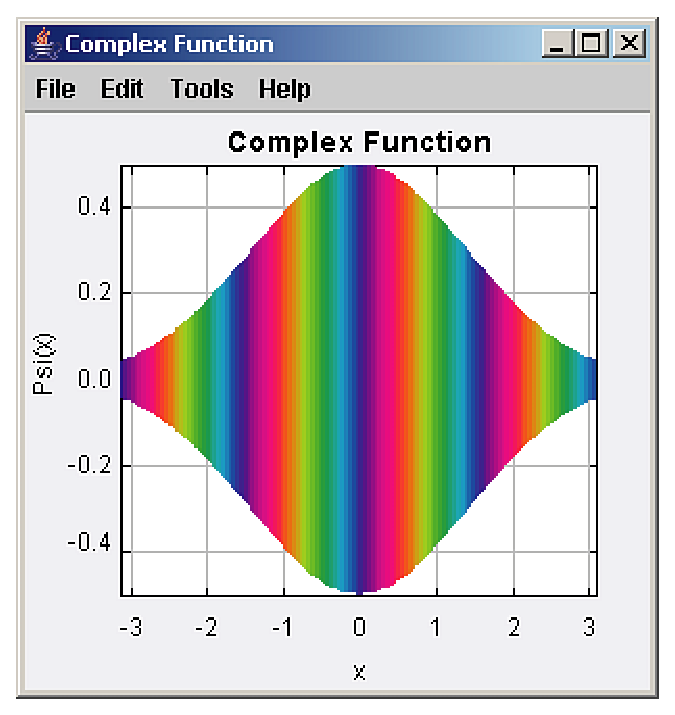
\includegraphics[scale=0.6]{phase}
\caption{\label{fig:phase}And here is your predicted phase diagram.}
\end{figure}

And here, I show the simulation results, which fall into three categories, 1) the frequency falloff can be explained by heterogeneity in length, 2) the steady state effective viscosity matches the theoretical prediction in a range of parameter space, 3) the network tearing time drops as the effective viscosity drops to 0

We have implemented a solution to the discretized form of our model equations.  

\begin{figure}[h!]
\centering
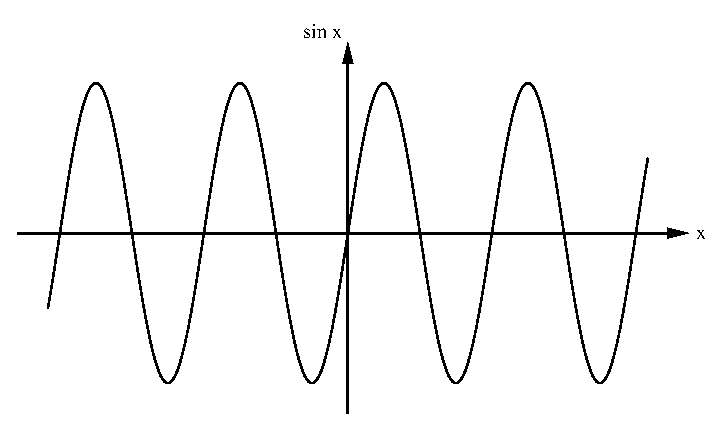
\includegraphics[scale=0.6]{sine}
\caption{\label{fig:sine}Show me a sine.}
\end{figure}

We can make figures bigger or smaller by scaling them. Figure~\ref{fig:sine}
has been scaled by 60\%.


\section{Simulation details}
And I think I'll probably include all the gory details of how my simulations work since I'll be wanting to have direct references to the code. 
\begin{verbatim}
double y0 = 10; // example of declaration and assignment statement
double v0 = 0;  // initial velocity
double t = 0;   // time
double dt = 0.01; // time step
double y = y0; // solved all problems
\end{verbatim}


\section{Discussion}

{\color{blue}{Finally I wax philosophical}},
{\color{green}{but}} {\color{cyan}{who is going pay for the ink?}}

\begin{thebibliography}{5}

\bibitem{latex}Helmut Kopka and Patrick W. Daly, \textsl{A Guide to
\LaTeX: Document Preparation for Beginners and Advanced Users} (Addison-Wesley, 2004), 4th ed.

\bibitem{website}Some useful links are
given at \url{<sip.clarku.edu/tutorials/TeX/>}.

\end{thebibliography}

\end{document}